\section{Introduction}\label{sec:intro}

\subsection{The project}\label{subsec:intro:project}

The motivation behind this project was to find a way, to apply deep learning methods to high energy particle physics.
The first thing I thought of was: "Can I train a computer to recognize a Higgs boson from plain experimental data from
the LHC?"
Luckily, there has already been a challenge by ATLAS in 2014 to improve their data research with machine learning
methods, called the Higgs boson machine learning challenge~\cite{adam2014learning}.

What my project is about after all is to take simulated ATLAS data from the CERN Open Data Portal to train a neural network.
The network is used for binary classification.
It classifies, whether a collision event contains the production of a Higgs boson (signal, s) or not (background, b).

\subsection{The data}\label{subsec:intro:data}

To do this project I need data from particle accelerator collision events that satisfies two key properties:
First, the collisions need to be done at a high enough center of mass energy to actually produce a Higgs boson.
This means that the collisions have to happen at energies of around $E_\text{COM}\sim 10^5 - 10^7$\;MeV.
Second, the events have to be labelled with the information, if a Higgs boson has been created during the collision.
Luckily, there is a dataset provided for the Higgs boson machine learning challenge which fulfills both criteria~\cite{atlas2014dataset}.
The dataset does not contain the full raw data from ATLAS though.
Due to the incredible size of the ATLAS detector and the number of parts, which take data, the raw data consists of $10^5 \sim 10^8$ dimensional datapoints.
This data is preprocessed a lot to bring it down to sizes which are easier to handle.
The actual dataset used for this project contains consists of 818238 events with 30 dimensions.\footnote{The full dataset contains even more dimensions, which are related to the challenge, but are not used in this project.}

\begin{figure}[t]
    \centering
    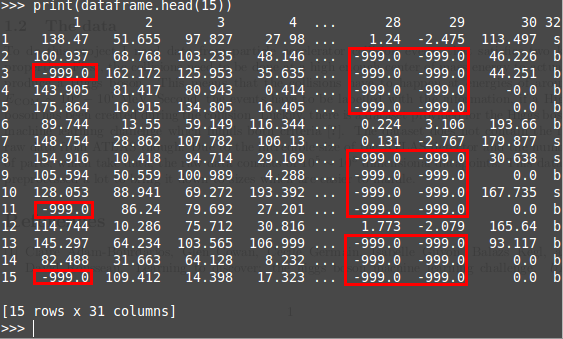
\includegraphics[width=\linewidth]{figures/datainfo_red.png}
    \caption{The first 15 datapoints from the dataset used. The red boxes mark missing data.}
    \label{fig:intro:datainfo}
\end{figure}

\subsubsection{Missing data}\label{subsubsec:intro:data:missing}

Figure \ref{fig:intro:datainfo} shows an excerpt from the dataset.
Note, that there are some points of data, which have a value of $-999.0$ in some columns, eventhough other datapoints are far off from that value.
Taking a closer look at the documentation of the data~\cite{adam2014learning} we see that some columns contain data, which is related to particle jets produced during the collision.
Events, in which no jets, or only one jet respectively, were produced, have missing data in some columns.
There were 568698 events, in which one or less jets were produced.
This results in those events having missing data in columns 5, 6, 7, 13, 27, 28 and 29.
During 320850 events there were no jets at all.
Those events have additional missing data in columns 24, 25 and 26.
To deal with this missing data, we will have to separate the events by the number of jets produced.

Unfortunately there is more missing data.
Column 1 contains data for the mass of a possible candidate for a Higgs boson.
The documentation for this columns says:\\
\\
\textit{"The estimated mass $m_H$ of the Higgs boson candidate, obtained through a probabilistic phase space integration (may be undefined if the topology of the event is too far from the expected topology)"}\\
\\
Therefore the missing data in this column is not directly related to the number of jets produced.
It is also not related to the label of the event (signal or background).
There are 122143 events with missing data in this column.
Thus this column will need to be treated separately.
